\documentclass[10pt]{beamer}

\usepackage{amssymb,amsthm}% http://ctan.org/pkg/amssymb
\newtheorem{proposition}{Proposition}
\setbeamertemplate{theorems}[numbered]
\usecolortheme[RGB={100,0,0}]{structure}
\setbeamercolor{block title}{use=structure,fg=white,bg=structure.fg!75!black}
\setbeamercolor{block body}{parent=normal text,use=block title,bg=block title.bg!10!bg}

\setbeamertemplate{footline}[frame number]

\usepackage{amsmath}
\DeclareMathOperator*{\argmax}{argmax}
\DeclareMathOperator*{\argmin}{argmin}

\usepackage{natbib}
\bibliographystyle{aea}

\usepackage{xcolor}
\usepackage{graphicx}
\usepackage{amsmath}
\usepackage{numprint}
\npdecimalsign{.}
\nprounddigits{3}
\usepackage{colortbl}
\usepackage{appendixnumberbeamer}
\usepackage{subfigure}
\usepackage{comment}

\usepackage{hyperref}
\usepackage{caption}
\setbeamerfont{caption}{size=\small}
\usetheme{Singapore}
\usecolortheme{beaver}

% for adding regression tables
\usepackage{dcolumn}
% column to line up decimals
\usepackage{booktabs,caption}
\captionsetup[table]{name=Table}
\setlength{\abovecaptionskip}{-1pt}
\setlength{\belowcaptionskip}{-1.5pt}
\usepackage[flushleft]{threeparttable} 
% The above two allow that last line with the dagger as a bottom note.

\usepackage{xcolor}
\definecolor{underbrace}{RGB}{30,199,166}
\newcommand{\textfrac}[1]{
  \begin{tabular}{@{}l@{}}#1\end{tabular}
}
\usepackage{tcolorbox}
\setbeamertemplate{caption}[numbered]

\title[ERPT]{Exchange Rate Pass-Through and Importers' Credit Constraints: Evidence From China}

\author[Li \& Lu]{Yao Amber LI\inst{*} \and Lingfei LU\inst{*}}

\institute[2024]{\inst{*} \small The Hong Kong University of Science and Technology}

\date{Australasian Trade Workshop (ATW) \\ \vspace{3mm} Christchurch, New Zealand \\ \vspace{4mm} March 17, 2024 }


\begin{document}
	
\begin{frame}
    \maketitle
    \centering
\end{frame}

\AtBeginSection[]
{
    \begin{frame}{Outline}
    \transfade
    \tableofcontents[sectionstyle=show/shaded,subsectionstyle=show/shaded/hide]
    \addtocounter{framenumber}{-1}
    \end{frame}
}

\section{Introduction}

\begin{frame}{What is Exchange Rate Pass-through?}
	\begin{itemize}
		\item Exchange rate shock is a key factor affecting international trade price fluctuations.
		\item The impact of bilateral exchange rate changes on prices denominated in buyers' and sellers' currencies may be asymmetric.
		\item Understanding the pattern of asymmetric prices has important implications for formulating macro policies, including monetary policy, inflation targeting, and the balance of payments.
	\end{itemize}
\end{frame}

\begin{frame}{What is Exchange Rate Pass-through?}
	\begin{itemize}
		\item Exchange rate pass-through (ERPT) is defined as \textbf{the elasticity of local price changes to exchange rate changes}.
		\item Exchange rate pass-through measures how exchange rate risk is shared between buyers and sellers of trade.
	\begin{figure}[htbp]
		\centering
		\includegraphics[width=0.9\columnwidth]{ERPT.jpg}
		\label{ERPT}
	\end{figure}
		\item In this example, we call $y$ (or $1-x$) as exchange rate pass-through.
	\end{itemize}
\end{frame}

\begin{frame}{Motivations}
	\begin{itemize}
		\item The degree of exchange rate pass-through to prices can vary significantly from firm to firm. But why? 
		\item The variation in financial constraints across firms and industries could affect international trade (e.g., \cite{manova2013}).
		\item It remains an open question whether \textbf{importers under financial constraints will behave differently} in price setting during exchange rate fluctuations compared to those less constrained.
	\end{itemize}
\end{frame}

\begin{frame}{Key Questions}
\textbf{Our research questions:}
	\begin{itemize}
		\item [1] What is the difference in exchange rate pass-through (ERPT) patterns between Chinese importers and exporters?
		\item [2] How do importing firms' (buyers') credit constraints affect the exchange rate pass-through?
		\item [3] What are the channels through which credit constraints affect import ERPT? What factors would enhance or mitigate this effect?
	\end{itemize}
\end{frame}

\begin{frame}{What We Do}
Using Chinese customs transaction records and firm-level data, we find:	
	\begin{enumerate}
		\item The average import exchange rate pass-through level in China is significantly less complete than the export one.
		\item Tighter financial constraints of importers will lead exchange rate pass-through to be more complete.
		\item Importers with higher sourcing diversity (who import a certain product from more sources) have a less complete ERPT and are less affected by credit constraints.
	\end{enumerate}	
\end{frame}

\begin{frame}{Contribution: Incomplete Exchange Rate Pass-through}
	\begin{itemize}
		\item We first contribute to the literature on \textbf{exchange rate disconnect}, particularly on firm-level evidence of incomplete price pass-through.
		\item Two milestone papers:
		\begin{itemize}
			\item \cite{bmm2012} (BMM): micro-level evidence of firm heterogeneity in response to real exchange rate shocks.
			\item \cite{aik2014} (AIK): firms with higher import intensity and larger market share have lower ERPT.
			\item More works: \cite{lmx2015}, \cite{chen2016}, \cite{garetto2016}, \cite{auer2016}, \cite{devereux2017}, etc.
		\end{itemize}
		\item Our contribution is to \textcolor{blue}{provide a novel perspective for exchange rate disconnect in emerging economies with immature financial markets}.
	\end{itemize}
\end{frame}

\begin{frame}{Contribution: Credit Constraints and Trade}
	\begin{itemize}
		\item Another important strand of literature discusses \textbf{the effects of firms’ credit constraints on international trade}.
            \begin{itemize}
                \item E.g.: \cite{kroszner2007} \cite{manova2013}, \cite{chaney2016}, \cite{feenstra2015}, \cite{manova-wei-zhang2015}, \cite{fan-lai-li2015}.
            \end{itemize}
		\item For the relationship between credit constraints and exchange rate pass-through, \cite{strasser2013} shows that financially constrained firms tend to pass more exchange rate shocks to prices.
		\begin{itemize}
			\item Two recent articles discussing credit constraints and ERPT with evidence from China, \cite{dai2021} and \cite{xu-guo2021}
		\end{itemize}
		\item We contribute to this literature by \textcolor{blue}{focusing on how importers behave under varying degrees of credit constraints and comparing their heterogeneous capacity to absorb exchange rate shocks}. 
	\end{itemize}	
\end{frame}

\section{Data and Measurements}

\begin{frame}{Data: Exchange Rates and Macro Variables}
	\begin{itemize}
		\item The bilateral nominal exchange rate is defined as the number of home currency units that can purchase a unit of foreign currency.
		\item The CPI-based real exchange rate ($RER_{ct}$) is defined as:
		$$
		RER_{ct}=NER_{ct} \cdot \frac{CPI_{ct}}{CPI_{CHN,t}}.
		$$
		\item An increase in $RER_{ct}$ means a real depreciation of the Chinese RMB against the
		foreign country’s $c$ currency.
		\item We also use the real GDP of trading partners computed with national accounts growth, $RGDP_{ct}$.
	\end{itemize}
\end{frame}

\begin{frame}{Data: Exchange Rates Fluctuations}
    \begin{figure}[htbp]
	\centering
	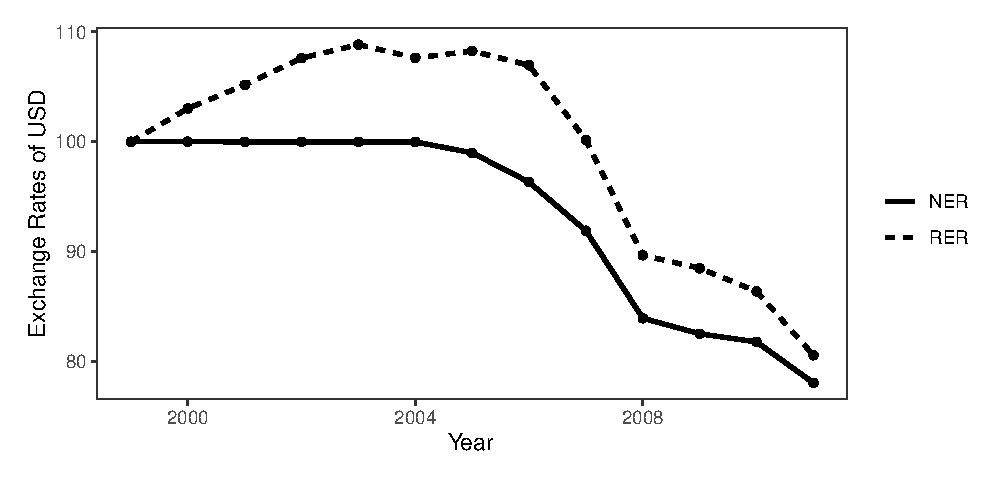
\includegraphics[width=0.65\columnwidth]{R/USD.eps}
        \label{fig.USD}
    \end{figure}
    \begin{figure}[htbp]
	\centering
	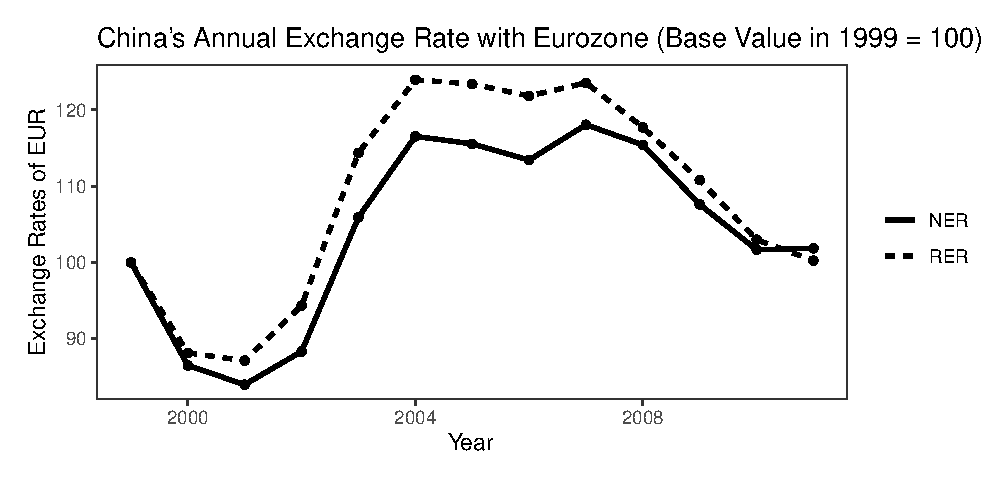
\includegraphics[width=0.65\columnwidth]{R/EUR.eps}
	\label{fig.EUR}
    \end{figure}
\end{frame}

\begin{frame}{Data: Firm-level and Customs data}
    \begin{itemize}
	\item Annual surveys of industrial enterprises from the National Bureau of Statistics of China
	\begin{itemize}
		\item Sample: all state-owned enterprises and above-scale firms (sales $>$5 million RMB), 1999 to 2007 
            \item Information: balance sheet variables, sales, employment, etc.
	\end{itemize}
        \medskip
        \item China Customs Records (from the General Administration of Customs of China)
        \begin{itemize}
            \item Sample: all exporting firms (except whole-sellers) in 2000-2011; matched manufacturing firms in 2000-2007 (baseline).
            \item Information: import and export values, quantities, product names and codes, source and destination countries, and firm types
	\end{itemize}
    \end{itemize}
\end{frame}

\begin{frame}{Data: Summary Statistics}
    \begin{table}[H]
        \centering
	\caption{Summary statistics for customs and firm data}
	\label{tab.summary.sample}
	\resizebox{\textwidth}{!}{
	\begin{threeparttable}
	\begin{tabular}{lcccccc}
		\toprule
            & \#observations & Mean & Median & {Std. Dev} & P10 & P90 \\
            \midrule
		\textbf{Panel A: Customs records} &       &       &       &       &       &  \\
		Export Price (RMB/unit) & 18,581,221 & 22007.45 & 30.1042 & 2229173 & 4.5645 & 556.4724 \\
		Annual Export Price Change & 11,400,795 & 0.0259 & 0.0060 & 0.6653 & -0.5001 & 0.5709 \\
		Import Price (RMB/unit) & 14,172,315 & 49519.78 & 111.0406 & 1411944 & 5.1594 & 10247.12 \\
		Annual Import Price Change  & 8,580,234 & 0.0236 & -0.0021 & 1.0171 & -0.8523 & 0.9388 \\
		\midrule
		\textbf{Panel B: Firm information} &       &       &       &       &       &  \\
		Sales Income (in 1000 RMB) & 1,745,511 & 78826.33 & 17630 & 714350.5 & 5318  & 111319 \\
		Employment (persons)& 1,745,511 & 262.95 & 108   & 964.64 & 30    & 500 \\
		Fixed Asset (in 1000 RMB) & 1,745,511 & 27437.2 & 4043  & 312024.8 & 573   & 36968 \\
		Operation Input (in 1000 RMB) & 1,745,511 & 61682.99 & 13971 & 562923.1 & 4035  & 168810 \\
		Current wage payable (in 1000 RMB) & 1,745,511 & 3730.16 & 1121  & 28699.16 & 266   & 6300 \\
		\midrule
		\textbf{Panel C: Matched sample} &       &       &       &       &       &  \\
		Export Price (RMB/unit) & 1,724,591 & 15960.54 & 28.7442 & 1806021 &  5.1482 & 380.3671 \\
		Annual Export Price Change & 1,724,591 & 0.0248 & 0.0056 & 0.7101 & -0.5251 & 0.5940 \\
		Import Price (RMB/unit) & 1,478,176 & 23573.29 & 81.9251 & 447447 & 4.9166 & 4169.39 \\
		Annual Import Price Change  & 1,478,176 & -0.0851 & -0.0018 & 1.4129 & -1.3406 &  1.1411 \\
		\bottomrule
	\end{tabular}
	\begin{tablenotes}
		\footnotesize
		\item Notes: This table shows the summary statistics of some important variables in our three major datasets. Panel A and panel C describe the total annual average prices and price changes for the whole and matched samples, respectively. The observations in panel A and panel C are at the firm-product-country-year level. The prices in panel A and panel C are in RMB. Panel B describes sales and costs information of Chinese manufacturing firms during 2000-2007. The money values in panel B are in thousands of RMB. The observations in panel B are at the firm-year level.
	\end{tablenotes}
	\end{threeparttable}
        }
    \end{table}
\end{frame}

\begin{frame}{Measures of Credit Constraints}
	\begin{itemize}
		\item Following \cite{manova-wei-zhang2015} and \cite{fan-lai-li2015}, we use sector-level financial vulnerability measures.
		\begin{enumerate}
			\item \textbf{External Finance Dependence ($ExtFin_j$)}: the share of capital expenditures not financed by operational cash flows.
			\item \textbf{Asset Tangibility ($Tang_j$)}: the share of the net value of tangible assets that firms can pledge as collateral in its total book value.
			\item \textbf{Inventory-to-sales Ratio ($Invent_j$)}: the production cycle duration in which firms need necessary working capital to maintain inventories.
		\end{enumerate}
		\item We construct the \textbf{first principal component} $FPC_j$ of external finance dependence and asset tangibility as an aggregate measure.
	\end{itemize}
\end{frame}

\begin{frame}{Measures of Credit Constraints}
    \begin{table}[H]
	\centering
	\caption{Summary statistics of measures of credit constraints}
	\label{tab.summary.credit}
	\resizebox{\textwidth}{!}{
	\begin{threeparttable}
		\begin{tabular}{lcccccc}
			\toprule
			& \multicolumn{1}{l}{\#observations} & \multicolumn{1}{l}{Mean} & \multicolumn{1}{l}{Median} & \multicolumn{1}{l}{Std. dev} & \multicolumn{1}{l}{P10} & \multicolumn{1}{l}{P90} \\
			\midrule
			\textbf{Panel A: US Measures} &       &       &       &       &       &  \\
			$FPC_{j}$ &  1,745,511 & 0 & -0.2707 & 1 & -1.0714  & 1.0727 \\
			$ExtFin_{j}$ & 1,745,511 & -0.0367 & -0.05 & 0.3112 & -0.25 & 0.28 \\
			$Tang_{j}$ & 1,745,511 & 0.3107 & 0.32 & 0.0944 & 0.1867 & 0.43 \\
			$Invent_{j}$ & 1,745,511 & 0.1594 & 0.1633  & 0.0292 & 0.115   & 0.1933 \\
			\midrule
			\textbf{Panel B: Chinese Measures} &       &       &       &       &       &  \\
			$FPC_{j}$ & 1,745,511 & 0 & 0.1021 & 1 & -1.0859  & 1.1619 \\
			$ExtFin_{j}$ & 1,745,511 & -0.6479 & -0.47 & 0.6747 & -1.32 & -0.1  \\
			$Tang_{j}$ & 1,745,511 & 0.3333 & 0.3269 & 0.0648 & 0.2391 & 0.4317 \\
			$Invent_{j}$ & 1,745,511 & 0.1103 & 0.1031  & 0.0275 & 0.0779   & 0.1348 \\
			$R\&D_{j}$ & 797,366 & 0.0168 & 0.0121 & 0.0142 & 0.0053  & 0.0282 \\
			\bottomrule
		\end{tabular}
		\begin{tablenotes}
			\footnotesize
			\item Notes: This table shows the summary statistics of credit constraint measures. Panel A describes the measures calculated using US data, while panel B shows the alternative measures from Chinese data.
			\end{tablenotes}
		\end{threeparttable}
	}
\end{table}
\end{frame}

\section{Empirical Analysis}

\begin{frame}{Baseline Estimation Equation}
	\begin{itemize}
		\item The first step goal is to estimate exchange rate pass-through as the elasticity of unit values changes to exchange rate changes.
		\begin{equation}
			\Delta \ln P_{i j c t}=\alpha+\beta \Delta \ln R E R_{c t}+\gamma \Delta \ln R G D P_{c t}+\xi_{i j c}+\tau_{t}+\varepsilon_{i j c t}
			\label{eq4.1}
		\end{equation}
            \begin{itemize}
                \item $P_{ijct}$: the price of the product $i$ bought (sold) by firm $j$ from (to) country $c$ in year $t$.
                \item $\xi_{ijc}$: the firm-product-country level fixed effects
                \item $\tau_t$: the year dummies, control for common macro-shocks across firms.
            \end{itemize}
		\item To deal with possible non-stationarity, we use the first difference of the logarithms for prices $\Delta \ln P_{i j c t}$, real exchange rates $\Delta \ln R E R_{c t}$ and real GDP $\Delta \ln R G D P_{c t}$ to represent annual rates of change.
	\end{itemize}
\end{frame}

\begin{frame}{Unit Value as Price}
	\begin{itemize}
		\item The customs records contain trade values (originally denominated by US dollars) and quantities $V_{ijct}$, and $Q_{ijct}$ for each HS6 product $i$, each firm $j$, from each country $c$, in each year $t$.
		\item The prices for export and import $P_{i j c t}$ are computed as unit values, both denominated by the Chinese RMB:
		$$
		P_{ijct}=\frac{V_{ijct}\cdot NER_{US,t}}{Q^{D}_{ijct}}
		$$
		\item Because product categories are highly subdivided, we believe that the unit value is an ideal proxy for the transaction price.
	\end{itemize}
\end{frame}

\begin{frame}{Results: Import Pass-through vs Export Pass-through}
    \begin{itemize}
	\item $\beta^{Import}$ measures the completeness of importers' ERPT.
        \begin{itemize}
            \item A higher $\beta$ means that Chinese importers face more volatile import RMB prices during exchange rate shocks.
        \end{itemize}
    \end{itemize}    
    \begin{table}[H]
	\centering
	\caption{Baseline estimations of exchange rate pass-through into import prices}
        \resizebox{0.8\columnwidth}{!}{
	\begin{threeparttable}
		\begin{tabular}{lcccc}
			\toprule
			& (1)   & (2)   & (3)   & (4) \\
			\midrule
			& \multicolumn{4}{c}{Import Prices: $\Delta \ln P_{ijct}$} \\
			& Whole & Matched & Top 50 & Top 20 \\
			\midrule
			$\Delta \ln RER_{ct}$ & 0.361*** & 0.732*** & 0.723*** & 0.658*** \\
			& (0.011) & (0.064) & (0.064) & (0.066) \\
			$\Delta \ln RGDR_{ct}$ & -0.180*** & 0.170 & 0.190 & 0.082 \\
			& (0.183) & (0.183) & (0.186) & (0.207) \\
                \midrule
			Year FE  & Yes   & Yes   & Yes   & Yes \\
			Firm-product-country FE & Yes   & Yes   & Yes   & Yes \\
			Observations & 7054033 & 1449210 & 1439301 & 1343150 \\
			\bottomrule
		\end{tabular}
		\begin{tablenotes}
			\footnotesize
			\item Notes: Robust standard errors clustered at firm level;  *, **, and *** indicate significance at 10\%, 5\%, and 1\% levels. Column (1) uses the whole customs data from 2000 to 2011. Column (2) uses the matched sample from 2000 to 2007. Columns (3) and (4) use sub-samples with only China's top 50 and top 20 partners ranked by total trade value. All regressions include firm-product-country fixed effects and year fixed effects. 
		\end{tablenotes}
	\end{threeparttable}
        }
	\label{tab.baseline}
    \end{table}
    \hyperlink{tab.baseline.exp}{\beamergotobutton{Export-Baseline}}
\end{frame}

\begin{frame}{Finding 1: Import Pass-through vs Export Pass-through}
	\begin{tcolorbox}[colback=blue!5!white, colframe=blue!75!black,title=Key Finding 1]
		\begin{itemize}
			\item The average exchange rate pass-through level for importers in China is less complete than that of exporters.
		\end{itemize}
	\end{tcolorbox}
	\begin{itemize}
		\item When RMB depreciates against the currencies of trading partners, export prices denominated in RMB will rise less significantly than import prices; when RMB appreciates, export prices in RMB will decrease only a little, but import costs will drop more.
		\item For firms that are highly dependent on imported inputs, the disadvantages of cost increases caused by depreciation may offset the competitive advantage of export prices.
	\end{itemize}
\end{frame}

\begin{frame}{Estimations with Credit Constraints}
	\begin{itemize}
		\item We study the credit constraint effects on exchange rate pass-through by including an interaction term of sectors’ financial vulnerability:
		\begin{equation}
			\begin{aligned}
				\Delta \ln P_{ijct}=&\alpha+\beta_{1} \Delta \ln RER_{ct}+\beta_{2} \Delta \ln RER_{ct} \cdot FV_{j} \\ &+\gamma \Delta \ln RGDP_{ct}+\xi_{ijc}+\tau_{t} +\varepsilon_{ijct}
			\end{aligned}
			\label{eq.credit}
		\end{equation}
		\begin{itemize}
		    \item $FV_{j}$: the financial vulnerability of the sector to which the firm $j$ belongs.
                \item $\beta_2$: the effect of credit constraints on exchange rate pass-through.
		\end{itemize}
		\item The overall ERPT for an importer $j$ is given by $\beta_{1} +\beta_{2} FV_j$ while for an exporter $j$ is given by $1-(\beta_{1} +\beta_{2} FV_j)$.
	\end{itemize}
\end{frame}

\begin{frame}{Results: Effects of Credit Constraints}
    \begin{table}[htb]
	\centering
	\caption{Effects of credit constraints on exchange rate pass-through into import prices}
        \resizebox{0.8\columnwidth}{!}{
	\begin{threeparttable}	
		\begin{tabular}{lcccc}
			\toprule
			& (1)   & (2)   & (3)   & (4) \\
			\midrule
			 & \multicolumn{4}{c}{Credit Constraints Measures} \\
			& FPC   & External Finance & Tangibility & Inventory \\
			\midrule
			$\Delta \ln RER_{ct}$ & 0.351*** & 0.493*** & 1.986*** & -0.930** \\
			& (0.075) & (0.065) & (0.258) & (0.420) \\
			$\Delta \ln RGDR_{ct}$ & 0.117 & 0.115 & 0.141 & 0.156 \\
			& (0.182) & (0.182) & (0.183) & (0.183) \\
			$\Delta \ln RER_{ct} \cdot FPC_{j}$ & 0.573*** &       &       &  \\
			& (0.089) &       &       &  \\
			$\Delta \ln RER_{ct} \cdot ExtFin_{j}$ &    & 1.749*** &       &  \\
			&   & (0.266) &       &  \\
			$\Delta \ln RER_{ct} \cdot Tang_{j}$ &   &       & -5.111*** &  \\
			&   &       & (0.960) &  \\
			$\Delta \ln RER_{ct} \cdot Invent_{j}$ &    &       &       & 9.536*** \\
			&   &       &       & (2.460) \\
                \midrule
			Year FE  & Yes   & Yes   & Yes   & Yes \\
			Firm-product-country FE & Yes   & Yes   & Yes   & Yes \\
			Observations & 1449210 & 1449210 & 1449210 & 1449210 \\
			\bottomrule
		\end{tabular}
		\begin{tablenotes}
			\footnotesize
			\item Notes: Robust standard errors clustered at firm level;  *, **, and *** indicate significance at 10\%, 5\%, and 1\% levels. Columns (1)-(4) use different measures of credit constraints calculated using U.S. data. All regressions include firm-product-country fixed effects and year fixed effects.
		\end{tablenotes}
	\end{threeparttable}
        }
	\label{tab.credit}
    \end{table}
    \hyperlink{tab.credit.exp}{\beamergotobutton{Export-Credit}}
\end{frame}

\begin{frame}{Finding 2: Effects of Credit Constraints}
	\begin{tcolorbox}[colback=blue!5!white, colframe=blue!75!black,title=Key Finding 2]
		\begin{itemize}
			\item Tighter financial constraints of importers will lead exchange rate pass-through to be more complete.
		\end{itemize}
	\end{tcolorbox}
	\begin{itemize}
		\item Exchange rate fluctuations are more likely to be reflected in unstable import costs for importers in financially vulnerable industries because they have weak bargaining power in the international market.
		\item \textit{Credit constraints expose Chinese manufacturing firms to greater exchange rate risk in international trade.}
	\end{itemize}
\end{frame}


\begin{frame}{Additional Firm-level Factors}
	To answer the third question, we introduce a vector $\mathbb{Z}_{jt}$ (or its lagged form $\mathbb{Z}_{jt-1}$) to include additional factors which may affect ERPT.
	\begin{enumerate}
		\item \textbf{Sourcing Diversity}: the number of source countries from which an importer $j$ imports a certain HS6 product type $i$. 
		\item \textbf{Markup}: estimated by the GMM method following \cite{dlw2012} and \cite{bkl2021}.
		\item \textbf{Market Share}: a firm’s value share in the import market, within a given HS6 product category.
		$$
		S^{D}_{ijct} \equiv \frac{v^{D}_{ijct}}{\sum_{j^{\prime} \in J_{ict}} v^{D}_{ij^{\prime}ct}}
		$$
	\end{enumerate}
\end{frame}

\begin{frame}{Estimations with Additional Factors}
	\begin{itemize}
		\item Estimation equations with additional factors $\mathbb{Z}_{jt}$:
		\begin{equation}
			\begin{aligned}
				\Delta \ln P_{ijct}=&\alpha+[\beta_{1}+ \beta_{2} \cdot FV_{j}+\beta_{3} \cdot {\mathbb{Z}_{jt}}'] \Delta \ln RER_{ct} \\&+\gamma \Delta \ln RGDP_{ct}+ {\mathbb{Z}_{jt}}' \eta+\xi_{ijc}+\tau_{t} +\varepsilon_{ijct}.
			\end{aligned}	
			\label{eq.add.control}
		\end{equation}
		\begin{equation}
			\begin{aligned}
				\Delta \ln P_{ijct}=&\alpha+[\beta_{1}+ \beta_{2} \cdot FV_{j}+\beta_{3} \cdot {\mathbb{Z}_{jt}}'+\beta_{4} \cdot FV_{j} \cdot {\mathbb{Z}_{jt}}'] \Delta \ln RER_{ct} \\ &+\gamma \Delta \ln RGDP_{ct}+ {\mathbb{Z}_{jt}}' \eta+\xi_{ijc}+\tau_{t} +\varepsilon_{ijct}.
			\end{aligned}	
			\label{eq.add.interaction}
		\end{equation}
		\item Now we focus on how \textbf{sourcing diversity} affects exchange rate pass-through for firms subject to different levels of credit constraints.
	\end{itemize}
\end{frame}

\begin{frame}{Results: Sources, Credit Constraints, and ERPT}
    \begin{table}[htbp]
	\centering
	\caption{Import sources, credit constraints, and exchange rate pass-through}
	\resizebox{\textwidth}{!}{
	\begin{threeparttable}
		\begin{tabular}{lcccccccc}
			\toprule
			& (1)   & (2)   & (3)   & (4) & (5)   & (6)   & (7)   & (8)   \\
			\midrule
			 & \multicolumn{4}{c}{Current Sources} & \multicolumn{4}{c}{Initial Sources} \\
			& \#Sources & \#Sources+ & \#Sources+ & \#Sources+	& \#Sources & \#Sources+ & \#Sources+ & \#Sources+ \\
			&       & FPC &External & Tangibility &  & FPC &External & Tangibility\\
			&       & &Finance & &       & &Finance &			\\
			\midrule
			$\Delta \ln RER_{ct}$ & 0.950*** & 0.550*** & 0.696*** & 2.375*** & 0.930*** & 0.548*** & 0.683*** & 2.282*** \\
			& (0.055) & (0.058) & (0.054) & (0.146) & (0.054) & (0.059) & (0.054) & (0.147) \\
			$\Delta \ln RGDR_{ct}$ & 0.143 & 0.080 & 0.080 & 0.108 & 0.143 & 0.082 & 0.082 & 0.109 \\
			& (0.126) & (0.126) & (0.126) & (0.126) & (0.126) & (0.126) & (0.126) & (0.126) \\
			$\#Source_{ijt}$ & -0.059*** & -0.059*** & -0.057*** & -0.081*** & -0.066*** & -0.071*** & -0.065*** & -0.076*** \\
			& (0.009) & (0.010) & (0.009) & (0.024) & (0.010) & (0.012) & (0.010) & (0.028) \\
			$\Delta \ln RER_{ct}*FPC_{j}*\#Source_{ijt}$ &    & -0.015** &       &       &       & -0.011 &       &  \\
			&   & (0.007) &       &       &       & (0.009) &       &  \\
			$\Delta \ln RER_{ct}*FPC_{j}$ &  & 0.670*** &       &       &       & 0.637*** &       &  \\
			&   & (0.046) &       &       &       & (0.047) &       &  \\
			$\Delta \ln RER_{ct}*ExtFin_{j}*\#Source_{ijt}$ &   &       & -0.064*** &       &       &       & -0.058** &  \\
			&   &       & (0.020) &       &       &       & (0.025) &  \\
			$\Delta \ln RER_{ct}*ExtFin_{j}$ &     &       & 2.113*** &       &       &       & 2.024*** &  \\
			&   &       & (0.137) &       &       &       & (0.140) &  \\
			$\Delta \ln RER_{ct}*Tang_{j}*\#Source_{ijt}$ &    &       &       & 0.049 &       &       &       & -0.005 \\
			&    &       &       & (0.098) &       &       &       & (0.116) \\
			$\Delta \ln RER_{ct}*Tang_{j}$ &   &       &       & -5.665*** &       &       &       & -5.374*** \\
			&  &       &       & (0.537) &       &       &       & (0.552) \\
                \midrule
			Year FE  & Yes   & Yes   & Yes   & Yes & Yes   & Yes   & Yes   & Yes\\
			Firm-product-country FE & Yes   & Yes   & Yes   & Yes & Yes   & Yes   & Yes   & Yes\\
			Observations & 1449210 & 1449210 & 1449210 & 1449210 & 1449210 & 1449210 & 1449210 & 1449210\\
			\bottomrule
		\end{tabular}
		\begin{tablenotes}
			\footnotesize
			\item Notes: Robust standard errors clustered at firm-product level; *, **, and *** indicate significance at 10\%, 5\%, and 1\% levels. Columns (1)-(4) use the number of source countries in the current year, while columns (5)-(8) use the number of source countries in the initial year. All regressions include firm-product-country fixed effects and year fixed effects.
		\end{tablenotes}
	\end{threeparttable}
	}
	\label{tab.source}
    \end{table}
    \hyperlink{tab.source.distance}{\beamergotobutton{Geographical Distance}}
\end{frame}

\begin{frame}{Finding 3: Sourcing Diversity, Credit Constraints, and ERPT}
	\begin{tcolorbox}[colback=blue!5!white, colframe=blue!75!black,title=Key Finding 3]
		\begin{itemize}
			\item Importers with a wider sourcing base (who import a certain product from more sources) have a less complete ERPT and are less affected by credit constraints.
		\end{itemize}
	\end{tcolorbox}
	\begin{itemize}
		\item If a firm can import the same product from more sources, it has more flexibility to escape the unfavorable exchange rate risk.
		\item A more diverse importer can either switch from one source to another to reduce costs (trade diversion effect), or make a more credible threat to negotiate a more stable price.
	\end{itemize}
\end{frame}

\section{Robustness}

\begin{frame}{Robustness 1: Alternative Measures of Credit Constraints}
    \begin{table}[H]
	\centering
	\caption{Robustness check: alternative credit constraints measures from Chinese data}
        \resizebox{0.85\columnwidth}{!}{
	\begin{threeparttable}
	\begin{tabular}{lccccc}
		\toprule
		& (1)   & (2)   & (3)   & (4) \\
		\midrule
		& \multicolumn{4}{c}{Measures of Credit Constraints from Chinese Data} \\
		  & External Finance & Tangibility & Inventory & R\&D Intensity \\
		\midrule
		$\Delta \ln RER_{ct}$  & 0.943*** & 3.427*** & -0.966*** & 0.215* \\
		 & (0.113) & (0.395) & (0.267) & (0.110) \\
		$\Delta \ln RGDP_{ct}$  & 0.154 & 0.142 & 0.168 & 0.160 \\
		 & (0.183) & (0.182) & (0.183) & (0.183) \\
		$\Delta \ln RER_{ct}$*$ExtFin_{j}$ & 0.327** &       &       &  \\
		& (0.134) &       &       &  \\
		$\Delta \ln RER_{ct}$*$Tang_{j}$ &        & -9.321*** &       &  \\
		&   &   (1.286) &       &  \\
		$\Delta \ln RER_{ct}*Invent_{j}$ &           &       & 14.919*** &  \\
		&       &       & (2.433) &  \\
		$\Delta \ln RER_{ct}*R\&D_{j}$ &         &       &       & 26.607*** \\
		&         &       &       & (5.291) \\
            \midrule
		Year FE  & Yes   & Yes   & Yes & Yes \\
		Firm-product-country FE   & Yes   & Yes   & Yes & Yes\\
		Observations & 1449210 & 1449210 & 1449210 & 1449210 \\
		\bottomrule
	\end{tabular}
	\begin{tablenotes}
		\footnotesize
		\item Notes: Robust standard errors clustered at firm level; *, **, and *** indicate significance at 10\%, 5\%, and 1\% levels. The dependent variable is the price change $\Delta \ln P_{ijct}$. Columns (1)-(4) use different measures of credit constraints calculated using Chinese data. All regressions include firm-product-country fixed effects and year fixed effects.
	\end{tablenotes}
	\end{threeparttable}
        }
        \label{tab.robust.credit}
    \end{table}
\end{frame}

\begin{frame}{Robustness 2: Alternative Transaction Samples}
    \begin{table}[H]
	\centering
	\caption{Robustness check: alternative samples excluding USD-pegged countries}
        \resizebox{0.85\columnwidth}{!}{
	\begin{threeparttable}
	\begin{tabular}{lcccc}
		\toprule
		& (1)   & (2)   & (3)   & (4) \\
		\midrule
		& \multicolumn{4}{c}{Excluding US Dollar Peg} \\
		& Baseline & FPC   & External Finance & Tangibility \\
		\midrule
		$\Delta \ln RER_{ct}$ & 0.849*** & 0.511*** & 0.642*** & 2.021*** \\
		& (0.086) & (0.086) & (0.081) & (0.266) \\
		$\Delta \ln RGDP_{ct}$ & 0.770*** & 0.678*** & 0.686*** & 0.710*** \\
		& (0.252) & (0.247) & (0.247) & (0.249) \\
		$\Delta \ln RER_{ct}$*$FPC_{j}$ &    & 0.526*** &       &  \\
            & & (0.086) &       &  \\
		$\Delta \ln RER_{ct}$*$ExtFin_{j}$ & &       & 1.590*** &  \\
		& &       & (0.255) &  \\
		$\Delta \ln RER_{ct}$*$Tang_{j}$ & &       &       & -4.753*** \\
		& &       &       & (0.933) \\
            \midrule
		Year FE  &   Yes    & Yes   & Yes   & Yes \\
		Firm-product-country FE &   Yes    & Yes   & Yes   & Yes \\
		Observations & 1147027 & 1147027 & 1147027 & 1147027 \\
		\bottomrule
	\end{tabular}
	\begin{tablenotes}
		\footnotesize
		\item Notes: Robust standard errors clustered at firm level; *, **, and *** indicate significance at 10\%, 5\%, and, 1\% levels. We do not include countries that use the U.S. dollar or currencies pegged to the U.S. dollar. Columns (2)-(4) use different measures of credit constraints calculated using U.S. data. All regressions include firm-product-country fixed effects and year fixed effects.
	\end{tablenotes}
        \end{threeparttable}
        }
        \label{tab.robust.nopeg}
    \end{table}
\end{frame}

\begin{frame}[label=robustness_other]{Other Robustness Checks}
    \begin{itemize}
	\item Robustness 3: trade type controls: (1) two-way traders vs pure importers and (2) ordinary trade vs processing trade \hyperlink{tab.robust.tradetype}{\beamergotobutton{Trade type}}
        \vfill
        \item Robustness 4: controls of firm ownership \hyperlink{tab.robust.ownership}{\beamergotobutton{Ownership}}
        \vfill
        \item Robustness 5: controls of firm-specific markup \hyperlink{tab.markup}{\beamergotobutton{Markup}}
        \vfill
        \item Robustness 6: (1) alternative fixed effects \hyperlink{tab.robust.fe}{\beamergotobutton{Alternative FEs}} and (2) cross-sectional estimation \hyperlink{tab.robust.crosec}{\beamergotobutton{Cross-sectional}}
    \end{itemize}
\end{frame}

\section{Discussion}

\begin{frame}{Discussion: Buyers' Market Share}
    \begin{itemize}
	\item How does an importer's market share in the market of a specific product affect its exchange rate pass-through?
        \item The ``import market share'' is defined as the fraction of a firm's import value to the total value imported by all Chinese importers from the same source $j$, within a given HS6 product $i$ in  year $t$:
        $$
        S_{ijct} \equiv \frac{v_{ijct}}{\sum_{j^{\prime} \in J_{ict}} v_{ij^{\prime}ct}}
        $$
        \item Can firm heterogeneity in market shares totally explain the effects of credit constraints on pass-through?
	\end{itemize}
\end{frame}

\begin{frame}{Result: Buyers' Market Share}
    \begin{table}[htb]
	\centering
	\caption{Heterogeneous Market Share, Credit Constraints, and Exchange Rate Pass-through}
        \resizebox{0.8\columnwidth}{!}{
	\begin{threeparttable}
		\begin{tabular}{lcccc}
			\toprule
			& (1)   & (2)   & (3)   & (4) \\
			\midrule
			&  Baseline    & FPC & External Finance& Tangibility        \\
			\midrule
			$\Delta \ln RER_{ct}$ & 0.832*** & 0.438*** & 0.579*** & 2.003*** \\
			& (0.070) & (0.079) & (0.069) & (0.258) \\
			$\Delta \ln RGDP_{ct}$ & 0.149 & 0.106 & 0.103 & 0.129 \\
			& (0.182) & (0.181) & (0.181) & (0.181) \\
			$\Delta \ln RER_{ct}*MS_{ijct}$ & -0.975*** & -0.728*** & -0.791*** & -0.782*** \\
			& (0.130) & (0.123) & (0.126) & (0.122) \\
			$\Delta \ln RER_{ct}$*$FPC_{j}$ &  & 0.555*** &       &  \\
			&  & (0.088) &       &  \\
			$\Delta \ln RER_{ct}$*$ExtFin_{j}$ &   &       & 1.705*** &  \\
			&  &       & (0.264) &  \\
			$\Delta \ln RER_{ct}$*$Tang_{j}$ &   &       &       & -4.859*** \\
			&   &       &       & (0.960) \\
			Year FE  & Yes  & Yes   & Yes   & Yes \\
			Firm-product-country FE & Yes    & Yes   & Yes   & Yes \\
			Market Share Control & Yes   & Yes   & Yes   & Yes \\
			Observations & 1449210  & 1449210 & 1449210 & 1449210 \\
			\bottomrule
		\end{tabular}
		\begin{tablenotes}
			\footnotesize
			\item Notes: Robust standard errors clustered at firm level; *, **, and *** indicate significance at 10\%, 5\%, and 1\%. Columns (2)-(4) use different measures of credit constraints calculated using U.S. data. All regressions include firm-product-country fixed effects and year fixed effects.
		\end{tablenotes}
	\end{threeparttable}
        }
	\label{tab.share}
    \end{table}
\end{frame}

\section{Conclusion}

\begin{frame}{Conclusion}
	\begin{itemize}
		\item This paper provides disaggregated level evidence for the incomplete exchange rate pass-through into import prices in China and reveals how importers’ financial constraints affect the pass-through.
		\item We find that:
		\begin{enumerate}
			\item The average exchange rate pass-through to import prices in China is around 70\%, which is less than the 95\% level for pass-through to export prices.
			\item Both import and export exchange rate pass-through are more complete for firms in industries with tighter credit constraints.
			\item Import source diversity can effectively reduce import price pass-through and offset the effects of credit constraints.
		\end{enumerate}
	\end{itemize}
\end{frame}

\begin{frame}[allowframebreaks,noframenumbering]
    \frametitle{References}
    \footnotesize
    \bibliography{setup/ref.bib}
\end{frame}

\appendix
\renewcommand{\thetable}{A.\arabic{table}}
\setcounter{table}{0}

\section*{More Tables}

\begin{frame}{Results: Import Pass-through vs Export Pass-through}
    \begin{itemize}
        \item However,  $\beta^{Export}$ means the "incompleteness" of exporters' ERPT. 
        \begin{itemize}
            \item A higher $\beta$ means exporters pass less exchange rate change to the local currency and have more volatile prices in the producer currency.
        \end{itemize}
    \end{itemize}
    \begin{table}[H]
	\centering
	\caption{Baseline Estimations of Exchange Rate Pass-Through to Export Prices}
        \resizebox{0.8\columnwidth}{!}{
	\begin{threeparttable}
		\begin{tabular}{lcccc}
			\toprule
			& (1)   & (2)   & (3)   & (4) \\
			\midrule
			& Whole & Matched & Top 50 & Top 20 \\
			\midrule
			$\Delta \ln RER_{ct}$ & 0.103*** & 0.060*** & 0.069*** & 0.123*** \\
			& (0.003) & (0.012) & (0.014) & (0.019) \\
			$\Delta \ln RGDR_{ct}$ &  -0.117*** & -0.085* & -0.145*** & -0.153** \\
			& (0.011) & (0.044) & (0.050) & (0.067) \\
			Year FE  & Yes   & Yes   & Yes   & Yes \\
			Firm-product-country FE & Yes   & Yes   & Yes   & Yes \\
			Observations & 10513011 & 1690715 & 1523544 & 1172135 \\
			\bottomrule
		\end{tabular}
		\begin{tablenotes}
			\footnotesize
			\item Notes: Robust standard errors clustered at firm level;  *, **, and *** indicate significance at 10\%, 5\%, and 1\% levels. Column (1) uses the whole customs data from 2000 to 2011. Column (2) uses the matched sample from 2000 to 2007. Columns (3) and (4) use sub-samples with only China's top 50 and top 20 partners ranked by total trade value. All regressions include firm-product-country fixed effects and year fixed effects. 
		\end{tablenotes}
	\end{threeparttable}
        }
	\label{tab.baseline.exp}
    \end{table}
    \hyperlink{tab.baseline}{\beamergotobutton{Back}}
\end{frame}

\begin{frame}{Results: Effects of Credit Constraints}
    \begin{table}[H]
	\centering
	\caption{Effects of Credit Constraints on Exchange Rate Pass-Through to Export Prices}
        \resizebox{0.8\columnwidth}{!}{
	\begin{threeparttable}	
		\begin{tabular}{lcccc}
			\toprule
			& (1)   & (2)   & (3)   & (4) \\
			\midrule
			& FPC   & External Finance & Tangibility & Inventory \\
			\midrule
			$\Delta \ln RER_{ct}$ & 0.074*** & 0.066*** & -0.034 & 0.162** \\
			& (0.013) & (0.013) & (0.036) & (0.071) \\
			$\Delta \ln RGDR_{ct}$ & -0.086* & -0.086* & -0.086* & -0.085* \\
			& (0.044) & (0.044) & (0.044) & (0.044) \\
			$\Delta \ln RER_{ct}*FPC_{j}$ & -0.031*** &       &       &  \\
			& (0.010) &       &       &  \\
			$\Delta \ln RER_{ct}*ExtFin_{j}$ &  & -0.090*** &       &  \\
			&  & (0.033) &       &  \\
			$\Delta \ln RER_{ct}*Tang_{j}$ &     &       & 0.354*** &  \\
			&     &       & (0.127) &  \\
			$\Delta \ln RER_{ct}*Invent_{j}$ &     &       &       & -0.593 \\
			&    &       &       & (0.407) \\
			Year FE  & Yes   & Yes   & Yes   & Yes \\
			Firm-product-country FE & Yes   & Yes   & Yes   & Yes \\
			Observations & 1690715 & 1690715 & 1690715 & 1690715 \\
			\bottomrule
		\end{tabular}
		\begin{tablenotes}
			\footnotesize
			\item Notes: Robust standard errors clustered at firm level; *, **, and *** indicate significance at 10\%, 5\%, and 1\% levels. Columns (1)-(4) use different measures of credit constraints calculated using U.S. data. All regressions include firm-product-country fixed effects and year fixed effects.
		\end{tablenotes}
	\end{threeparttable}
        }
	\label{tab.credit.exp}
    \end{table}
    \hyperlink{tab.credit}{\beamergotobutton{Back}}
\end{frame}

\begin{frame}{Results: Geographical Distance}
    \begin{table}[htbp]
	\centering
	\caption{Import Sources, Credit Constraints, and Exchange Rate Pass-Through: Geographical Distance}
	\resizebox{\textwidth}{!}{
		\begin{threeparttable}
			\begin{tabular}{lcccccccc}
				\toprule
				& (1)   & (2)   & (3)   & (4) & (5)   & (6)   & (7)   & (8)   \\
				\midrule
				& \multicolumn{4}{c}{Simple Distance} & \multicolumn{4}{c}{Population-weighted Distance} \\
				&       & FPC &External & Tangibility &       & FPC &External & Tangibility\\
				&       & &Finance & &       & &Finance &			\\
				\midrule
				$\Delta \ln RER_{ct}$ & 1.099*** & 0.494*** & 0.688*** & 2.652*** & 1.099*** & 0.477*** & 0.675*** & 2.680*** \\
				& (0.107) & (0.117) & (0.101) & (0.417) & (0.112) & (0.120) & (0.104) & (0.432) \\
				$\Delta \ln RGDR_{ct}$ & 0.039 & 0.006 & -0.007 & 0.030 & 0.051 & 0.017 & 0.003 & 0.041 \\
				& (0.189) & (0.188) & (0.188) & (0.189) & (0.189) & (0.188) & (0.188) & (0.189) \\
				$ Distance_{ijt}$ & -0.090*** & -0.039** & -0.055*** & -0.188*** & -0.090*** & -0.036** & -0.052*** & -0.194*** \\
				& (0.018) & (0.015) & (0.015) & (0.062) & (0.019) & (0.016) & (0.016) & (0.067) \\
				$\Delta \ln RER_{ct}*FPC_{j}*Distance_{ijt}$ &    & -0.063*** &       &       &       & -0.068*** &       &  \\
				&   & (0.020) &       &       &       & (0.022) &       &  \\
				$\Delta \ln RER_{ct}*FPC_{j}$ &    & 0.805*** &       &       &       & 0.827*** &       &  \\
				&     & (0.141) &       &       &       & (0.146) &       &  \\
				$\Delta \ln RER_{ct}*ExtFin_{j}*Distance_{ijt}$ &    &       & -0.222*** &       &       &       & -0.242*** &  \\
				&    &       & (0.057) &       &       &       & (0.061) &  \\
				$\Delta \ln RER_{ct}*ExtFin_{j}$ &    &       & 2.653*** &       &       &       & 2.738*** &  \\
				&    &       & (0.418) &       &       &       & (0.433) &  \\
				$\Delta \ln RER_{ct}*Tang_{j}*Distance_{ijt}$ &     &       &       & 0.441** &       &       &       & 0.465** \\
				&    &       &       & (0.206) &       &       &       & (0.221) \\
				$\Delta \ln RER_{ct}*Tang_{j}$ &    &       &       & -6.572*** &       &       &       & -6.697*** \\
				&     &       &       & (1.543) &       &       &       & (1.590) \\
				Year FE  & Yes   & Yes   & Yes   & Yes & Yes   & Yes   & Yes   & Yes\\
				Firm-product-country FE & Yes   & Yes   & Yes   & Yes & Yes   & Yes   & Yes   & Yes\\
				Observations & 1449210 & 1449210 & 1449210 & 1449210 & 1449210 & 1449210 & 1449210 & 1449210\\
				\bottomrule
			\end{tabular}
			\begin{tablenotes}
				\footnotesize
				\item Notes:Robust standard errors clustered at firm level; *, **, and *** indicate significance at 10\%, 5\%, and 1\% levels. Columns (1)-(4) use the simple distance between the most populated cities of the two countries while columns (5)-(8) use the population-weighted harmonic mean distance between the two countries. All regressions include firm-product-country fixed effects and year fixed effects.
			\end{tablenotes}
		\end{threeparttable}
	}
	\label{tab.source.distance}
    \hyperlink{tab.source}{\beamergotobutton{Back}}
    \end{table}
\end{frame}

\begin{frame}{Robustness: Trade Type Controls}
    \begin{table}[htbp]
	\centering
	\caption{Robustness check: trade type controls for two-way traders or processing trade}
        \resizebox{\textwidth}{!}{
	\begin{threeparttable}
		\begin{tabular}{lcccccccc}
			\toprule
			& (1)   & (2)   & (3)   & (4) &  (5)  &  (6)   & (7)   & (8)\\
			\midrule
			& \multicolumn{4}{c}{Two-way Traders Controls} & \multicolumn{4}{c}{Processing Trade Controls}\\
			& Baseline & FPC & External Finance & Tangibility & Baseline & FPC & External Finance & Tangibility\\
			\midrule
			$\Delta \ln RER_{ct}$ & 0.732*** & 0.352*** & 0.493*** & 1.986*** & 0.736*** & 0.355*** & 0.496*** & 2.000*** \\
			& (0.064) & (0.075) & (0.065) & (0.258) & (0.064) & (0.075) & (0.065) & (0.256) \\
			$\Delta \ln RGDP_{ct}$ & 0.170 & 0.117 & 0.116 & 0.141 & 0.149 & 0.096 & 0.096 & 0.120 \\
			& (0.184) & (0.182) & (0.182) & (0.183) & (0.183) & (0.182) & (0.182) & (0.183) \\
			$\Delta \ln RER_{ct}$*$FPC_{j}$ &   & 0.573*** &       &       &       & 0.574*** &       &  \\
			&   & (0.088) &       &       &       & (0.088) &       &  \\
			$\Delta \ln RER_{ct}$*$ExtFin_{j}$ &    &       & 1.749*** &       &       &       & 1.746*** &  \\
			&     &       & (0.266) &       &       &       & (0.264) &  \\
			$\Delta \ln RER_{ct}$*$Tang_{j}$ &     &       &       & -5.111*** &       &       &       & -5.151*** \\
			&     &       &       & (0.959) &       &       &       & (0.952) \\
			Year FE  &  Yes   & Yes   & Yes   & Yes &  Yes   & Yes   & Yes   & Yes\\
			Firm-product-country FE &  Yes   & Yes   & Yes   & Yes &  Yes   & Yes   & Yes   & Yes\\
			Two-way trade control &  Yes   & Yes   & Yes   & Yes & No & No & No & No\\
			Processing trade controls & No & No & No & No &  Yes   & Yes   & Yes  & Yes \\
			Observations & 1449210 & 1449210 & 1449210 & 1449210 & 1449210 & 1449210 & 1449210 & 1449210\\
			\bottomrule
		\end{tabular}
		\begin{tablenotes}
			\footnotesize
			\item Notes: Robust standard errors clustered at firm level; *, **, and *** indicate significance at 10\%, 5\%, and 1\% levels. The dependent variable is the price change $\Delta \ln P_{ijct}$. We only include those firms that simultaneously import and export during the same year. Columns (2)-(4) use different measures of credit constraints calculated using U.S. data. All regressions include firm-product-country fixed effects and year fixed effects.
		\end{tablenotes}
	\end{threeparttable}
        }
	\label{tab.robust.tradetype}
    \end{table}
    \hyperlink{robustness_other}{\beamergotobutton{Back}}
\end{frame}

\begin{frame}{Robustness: Ownership Controls}
    \begin{table}[htbp]
	\centering
	\caption{Robustness check: ownership controls for registration type and affiliation}
        \resizebox{\textwidth}{!}{
	\begin{threeparttable}
		\begin{tabular}{lcccccccc}
			\toprule
			& (1)   & (2)   & (3)   & (4) &  (5)  &  (6)  & (7)  & (8)\\
			\midrule
			& \multicolumn{4}{c}{Ownership registration controls} & \multicolumn{4}{c}{Affiliation controls}\\
			& Baseline & FPC   & External Finance & Tangibility & Baseline & FPC & External Finance & Tangibility\\
			\midrule
			$\Delta \ln RER_{ct}$ & 0.879*** & 0.617*** & 0.696*** & 1.629*** & 0.879*** & 0.616*** & 0.696*** & 1.633*** \\
			& ((0.035) & (0.044) & (0.037) & (0.154) & (0.035) & (0.044) & (0.037) & (0.154) \\
			$\Delta \ln RGDP_{ct}$ & 0.593*** & 0.564*** & 0.554*** & 0.583*** & 0.596*** & 0.567*** & 0.558*** & 0.586*** \\
			& (0.102) & (0.102) & (0.101) & (0.102) & (0.103) & (0.102) & (0.102) & (0.102) \\
			$\Delta \ln RER_{ct}$*$FPC_{j}$ &    & 0.403*** &       &       &       & 0.405*** &       &  \\
			&  & (0.053) &       &       &       & (0.053) &       &  \\
			$\Delta \ln RER_{ct}$*$ExtFin_{j}$ &    &       & 1.356*** &       &       &       & 1.362*** &  \\
			&   &       & (0.155) &       &       &       & (0.155) &  \\
			$\Delta \ln RER_{ct}$*$Tang_{j}$ &     &       &       & -3.039*** &       &       &       & -3.057*** \\
			&   &       &       & (0.581) &       &       &       & (0.581) \\
			Year FE  &  Yes   & Yes   & Yes   & Yes & Yes   & Yes   & Yes   & Yes\\
			Product-country FE &  Yes   & Yes   & Yes   & Yes & Yes   & Yes   & Yes   & Yes\\
			Sales income control &  Yes   & Yes   & Yes   & Yes & Yes   & Yes   & Yes   & Yes\\
			Ownership registration control &  Yes   & Yes & Yes  & Yes & No & No & No & No\\
			Affiliation control & No & No & No & No &  Yes  & Yes & Yes  & Yes \\
			Observations & 1449168 & 1449168 & 1449168 & 1449168 & 1449168 & 1449168 & 1449168 & 1449168\\
			\bottomrule
		\end{tabular}
		\begin{tablenotes}
			\footnotesize
			\item Notes: Robust standard errors clustered at firm level; *, **, and *** indicate significance at 10\%, 5\%, and 1\% levels. Columns (1)-(4) include controls of registration type while columns (5)-(8) include controls of affiliation. All regressions include firm-product-country fixed effects and year fixed effects.
		\end{tablenotes}
	\end{threeparttable}
        }
	\label{tab.robust.ownership}
    \end{table}
    \hyperlink{robustness_other}{\beamergotobutton{Back}}
\end{frame}

\begin{frame}{Robustness: Markup Controls}
    \begin{table}[H]
	\centering
	\caption{Robustness check: markup controls}
        \resizebox{0.8\textwidth}{!}{
	\begin{threeparttable}
		\begin{tabular}{lcccc}
			\toprule         
			& (1)   & (2)   & (3)   & (4)     \\
			\midrule
			& Baseline & FPC & External Finance & Tangibility\\
			\midrule
			$\Delta \ln RER_{ct}$ & 0.763** & 0.543* & 0.725** & 2.121*** \\
			& (0.331) & (0.322) & (0.322) & (0.426) \\
			$\Delta \ln RGDP_{ct}$ & 0.260*	& 0.203 & 0.201 & 0.230*\\
			& (0.137) & (0.137) & (0.137) & (0.137)  \\
			$\Delta \ln RER_{ct}$*$FPC_{j}$ &   & 0.589*** &       &  \\
			&   & (0.094) &       &  \\
			$\Delta \ln RER_{ct}$*$ExtFin_{j}$ &     &       & 1.786*** &  \\
			&   &       & (0.284) &  \\
			$\Delta \ln RER_{ct}$*$Tang_{j}$  &     &       &       & -5.272*** \\
			&    &       &       & (1.015) \\
                $\Delta \ln RER_{ct}$*$Markup_{jt}$ &  -0.030 & -0.161 & -0.186 & -0.080 \\
			&   (0.240) & (0.236) & (0.238) & (0.237) \\
			Year FE  & Yes   & Yes   & Yes   & Yes       \\
			Firm-product-country FE & Yes   & Yes   & Yes   & Yes       \\
			Markup Control & Yes   & Yes   & Yes   & Yes       \\
			Observations & 1343563 & 1343563 & 1343563 & 1343563  \\
			\bottomrule
		\end{tabular}
		\begin{tablenotes}
			\footnotesize
			\item Notes: Robust standard errors clustered at firm level; *, **, and *** indicate significance at 10\%, 5\% and 1\%. All columns include firm-level markup levels and their interactions with $\Delta \ln RER_{ct}$ as controls. Firm-level markup is estimated using the method of \cite{dlw2012}. Columns (2)-(4) use different measures of credit constraints calculated using U.S. data. All regressions include firm-product-country fixed effects and year fixed effects.
		\end{tablenotes}
	\end{threeparttable}
        }
        \label{tab.markup}
    \end{table}
    \hyperlink{robustness_other}{\beamergotobutton{Back}}
\end{frame}

\begin{frame}{Robustness: Alternative Fixed Effects}
    \begin{table}[htbp]
	\centering
	\caption{Robustness check: alternative fixed effects}
        \resizebox{\textwidth}{!}{
	\begin{threeparttable}
		\begin{tabular}{lcccccccc}
			\toprule
			& (1)   & (2)   & (3)   & (4) &  (5)  &  (6)  & (7)  & (8)\\
			\midrule
			& \multicolumn{4}{c}{Firm-year FE + Product FE + Country FE} & \multicolumn{4}{c}{Firm-year FE + Product-Country FE}\\
			& Baseline & FPC   & External Finance & Tangibility & Baseline & FPC & External Finance & Tangibility\\
			\midrule
			$\Delta \ln RER_{ct}$ & 0.670*** & 0.567*** & 0.593*** & 0.946*** & 0.691*** & 0.626*** & 0.639*** & 0.841*** \\
                & (0.035) & (0.042) & (0.037) & (0.111) & (0.036) & (0.044) & (0.038) & (0.120) \\
			$\Delta \ln RGDP_{ct}$ & 0.753*** & 0.758*** & 0.759*** & 0.755*** & 0.788*** & 0.789*** & 0.790*** & 0.788*** \\
			& (0.108) & (0.108) & (0.108) & (0.108) & (0.112) & (0.112) & (0.112) & (0.112) \\
			$\Delta \ln RER_{ct}$*$FPC_{j}$ &  & 0.139*** &       &       &       & 0.086** &       &  \\
			&  & (0.035) &       &       &       & (0.038) &       &  \\
			$\Delta \ln RER_{ct}$*$ExtFin_{j}$ &   &       & 0.456*** &       &       &       & 0.297*** &  \\
			&  &       & (0.095) &       &       &       & (0.104) &  \\
			$\Delta \ln RER_{ct}$*$Tang_{j}$ &   &       &       & -1.139*** &       &       &       & -0.623 \\
			&   &       &       & (0.429) &       &       &       & (0.467) \\
			Firm-year FE  &  Yes   & Yes   & Yes & Yes & Yes & Yes & Yes & Yes\\
			Product-country FE & No & No & No & No & Yes & Yes & Yes & Yes\\
			Country FE &  Yes   & Yes   & Yes   & Yes & No & No & No & No\\
			Product FE &  Yes   & Yes   & Yes   & Yes & No & No & No & No\\
			Observations & 1428072 & 1428072 & 1428072 & 1428072 & 1416558 & 1416558 & 1416558 & 1416558 \\
			\bottomrule
		\end{tabular}
		\begin{tablenotes}
			\footnotesize
			\item Notes: Robust standard errors clustered at firm level; *, **, and *** indicate significance at 10\%, 5\%, and 1\% levels. Columns (1)-(4) include firm-year, country, and product fixed effects.  Columns (5)-(8) include firm-year and country-product fixed effects.
		\end{tablenotes}
	\end{threeparttable}
        }
	\label{tab.robust.fe}
    \end{table}
    \hyperlink{robustness_other}{\beamergotobutton{Back}}
\end{frame}

\begin{frame}{Robustness: Cross-sectional Estimations}
    \begin{table}[htbp]
	\centering
	\caption{Robustness check: cross-sectional estimations}
        \resizebox{\textwidth}{!}{
	\begin{threeparttable}
		\begin{tabular}{lcccccccc}
			\toprule
			& (1)   & (2)   & (3)   & (4) &  (5)  &  (6)  & (7)  & (8)\\
			\midrule
			& \multicolumn{4}{c}{One-year sample} & \multicolumn{4}{c}{Between estimator}\\
			& Baseline & FPC   & External Finance & Tangibility & Baseline & FPC & External Finance & Tangibility\\
			\midrule
			$\Delta \ln RER_{ct}$ & 2.841*** & 2.463*** & 2.541*** & 3.797*** & 0.766*** & 0.693*** & 0.714*** & 0.973*** \\
			& (0.143) & (0.175) & (0.160) & (0.405) & (0.039) & (0.047) & (0.043) & (0.117) \\
			$\Delta \ln RGDP_{ct}$ & -1.133*** & -1.207*** & -1.234*** & -1.159*** & -0.348*** & -0.359*** & -0.359*** & -0.354*** \\
			& (0.315) & (0.315) & (0.316) & (0.315) & (0.096) & (0.096) & (0.096) & (0.096) \\
			$\Delta \ln RER_{ct}$*$FPC_{j}$ &   & 0.483*** &       &       &       & 0.102*** &       &  \\
			&   & (0.129) &       &       &       & (0.037) &       &  \\
			$\Delta \ln RER_{ct}$*$ExtFin_{j}$ &   &       & 1.673*** &       &       &       & 0.326*** &  \\
			&  &       & (0.401) &       &       &       & (0.112) &  \\
			$\Delta \ln RER_{ct}$*$Tang_{j}$ &   &       &       & -4.006** &       &       &       & -0.852* \\
			&   &       &       & (1.587) &       &       &       & (0.456) \\
			Firm-product FE &  Yes   & Yes   & Yes   & Yes &Yes   & Yes   & Yes   & Yes\\
			Observations & 239338 & 239338 & 239338 & 239338 & 706717 & 706717 & 706717 & 706717 \\
			\bottomrule
		\end{tabular}
		\begin{tablenotes}
			\footnotesize
			\item Notes: Robust standard errors clustered at firm level; *, **, and *** indicate significance at 10\%, 5\%, and 1\% levels. Columns (1)-(4) report results using a one-year sample in 2007, while columns (5)-(8) report results using between estimators (average over 2000-2007). All regressions include firm-product fixed effect.
		\end{tablenotes}
	\end{threeparttable}
        }
	\label{tab.robust.crosec}
    \end{table}
    \hyperlink{robustness_other}{\beamergotobutton{Back}}
\end{frame}

\end{document}